% 2006 湖南文科候选卷 Q18；两个共底正四棱锥，按源图结构重绘，不按比例。
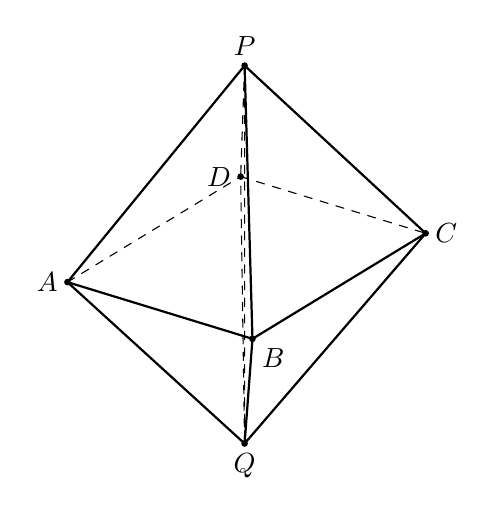
\begin{tikzpicture}[line cap=round,line join=round]
  \coordinate (A) at (-2.2,0);
  \coordinate (B) at (0.15,-0.72);
  \coordinate (C) at (2.35,0.62);
  \coordinate (D) at (0.0,1.34);
  \coordinate (P) at (0.05,2.75);
  \coordinate (Q) at (0.05,-2.05);

  % Hidden back edges and the common altitude line.
  \draw[dashed] (A)--(D) (D)--(C);
  \draw[dashed] (P)--(D) (Q)--(D) (P)--(Q);

  % Visible base and lateral edges.
  \draw[thick] (A)--(B)--(C);
  \draw[thick] (P)--(A) (P)--(B) (P)--(C);
  \draw[thick] (Q)--(A) (Q)--(B) (Q)--(C);

  \foreach \pt in {A,B,C,D,P,Q}{\fill (\pt) circle[radius=1.2pt];}
  \node[left] at (A) {$A$};
  \node[below right] at (B) {$B$};
  \node[right] at (C) {$C$};
  \node[left] at (D) {$D$};
  \node[above] at (P) {$P$};
  \node[below] at (Q) {$Q$};
\end{tikzpicture}
